\let\negmedspace\undefined
\let\negthickspace\undefined
\documentclass[journal]{IEEEtran}
\usepackage[a5paper, margin=10mm, onecolumn]{geometry}
\usepackage{tfrupee} % Include tfrupee package

\setlength{\headheight}{1cm} 
\setlength{\headsep}{0mm}     

\usepackage{gvv-book}
\usepackage{gvv}
\usepackage{cite}
\usepackage{amsmath,amssymb,amsfonts,amsthm}
\usepackage{algorithmic}
\usepackage{graphicx}
\usepackage{textcomp}
\usepackage{xcolor}
\usepackage{txfonts}
\usepackage{listings}
\usepackage{enumitem}
\usepackage{mathtools}
\usepackage{gensymb}
\usepackage{comment}
\usepackage[breaklinks=true]{hyperref}
\usepackage{tkz-euclide} 
\usepackage{listings}
\def\inputGnumericTable{}                                 
\usepackage[latin1]{inputenc}                                
\usepackage{color}                                            
\usepackage{array}                                            
\usepackage{longtable}                                       
\usepackage{calc}                                             
\usepackage{multirow}                                         
\usepackage{hhline}                                           
\usepackage{ifthen}                                           
\usepackage{lscape}
\usepackage{circuitikz}
\tikzstyle{block} = [rectangle, draw, fill=blue!20, 
    text width=4em, text centered, rounded corners, minimum height=3em]
\tikzstyle{sum} = [draw, fill=blue!10, circle, minimum size=1cm, node distance=1.5cm]
\tikzstyle{input} = [coordinate]
\tikzstyle{output} = [coordinate]


\begin{document}

\bibliographystyle{IEEEtran}
\vspace{3cm}

\title{5.3.30}
\author{AI25BTECH11036-SNEHAMRUDULA}
 \maketitle
{\let\newpage\relax\maketitle}
\renewcommand{\thefigure}{\theenumi}
\renewcommand{\thetable}{\theenumi}
\setlength{\intextsep}{10pt} 
\numberwithin{equation}{enumi}
\numberwithin{figure}{enumi}
\renewcommand{\thetable}{\theenumi}
\textbf{Q.}\;
\noindent\textbf{Question.}\;
Solve the system of linear equations 
\[
7u+2v=11,\qquad 4u-v=2 .
\]

\noindent\textbf{Solution.}
\begingroup
\setcounter{equation}{0}
\renewcommand{\theequation}{\arabic{equation}}

\begin{equation}
\myvec{7 & 2\\[2pt] 4 & -1}\,\myvec{u\\ v}=\myvec{11\\ 2},
\qquad
\vec A=\myvec{7 & 2\\ 4 & -1},\;
\vec p=\myvec{u\\ v},\;
\vec b=\myvec{11\\ 2}. 
\end{equation}

Since
\begin{equation}
\det(\vec A)=-15\neq 0,
\end{equation}
the unique solution is \(\vec p=\vec A^{-1}\vec b\) with
\begin{equation}
\vec A^{-1}=\frac{1}{\det(\vec A)}
\myvec{-1 & -2\\[2pt] -4 & 7}
=\frac{-1}{15}\myvec{-1 & -2\\ -4 & 7}.
\end{equation}
Hence
\begin{equation}
\vec p
= \frac{-1}{15}\myvec{-1 & -2\\ -4 & 7}\myvec{11\\ 2}
= \frac{-1}{15}\myvec{-15\\ -30}
= \myvec{1\\ 2}.
\end{equation}

Therefore,
\begin{equation}
u=1,\qquad v=2.
\end{equation}
\endgroup
and the number of unknowns is also \(3\), the system has a \textbf{unique solution}.
\endgroup
\begin{figure}[h!]
    \centering
    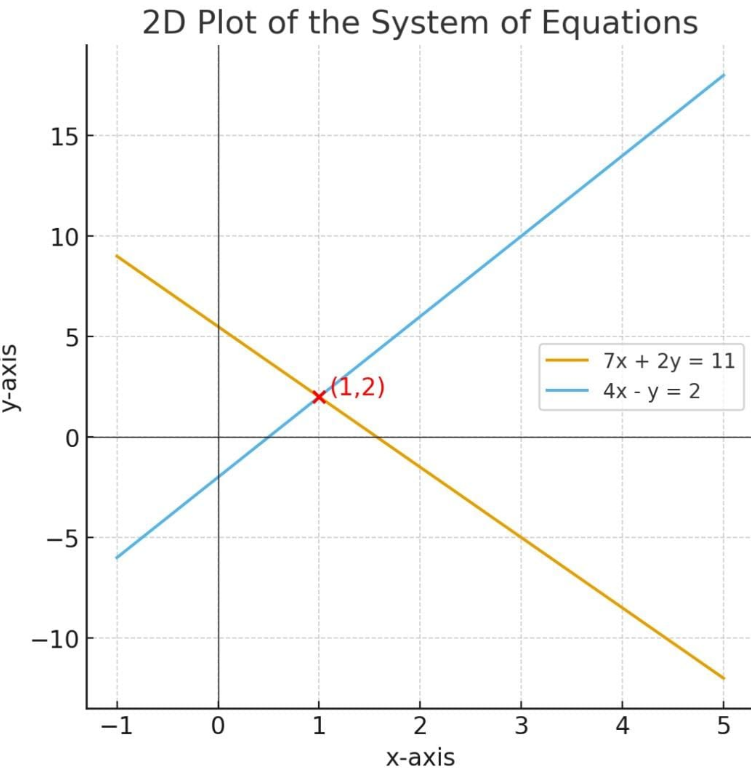
\includegraphics[height=0.5\textheight, keepaspectratio]{fig5.3.30}
    \label{figure_1}
\end{figure}
 
\end{document}